\chapter[Comunicação]{Comunicação}
\section{Algoritmo da Rede de Comunicação}
\subsection{Transceptor RF nRF24LE1}
Essa seção de dedica a especificação do módulo RF a ser utilizado, tratando sobre os protocolos de comunicação das camadas OSI já implementadas, camadas Física e de Enlace. O modelo OSI (Open System Interconnection) é um modelo de rede de computadores amplamente utilizado em aplicações de telecomunicações.Trata-se de um padrão e/ou arquitetura para protocolos de comunicação. O modelo secciona redes de computadores em sete camadas, com objetivo de que a cada camada seja atribuída uma funcionalidade assinalada por um protocolo específico. As sete camadas do sistema OSI são: Física, Enlace, Rede, Transporte, Sessão, Apresentação e Aplicação. Nesta sessão, com dito anteriormente, vamos tratar mais especificamente das camadas Física e de Enlace, que são implementadas no módulo RF nRF24LE1.

\subsubsection{Camada Física}

Na camada física são tratados dos itens de princípios físicos de comunicação, como taxas de transferência de dados, frequência de recepção e transmissão, largura de banda do sinal, filtros de recepção e afins. Dessa forma, o módulo RF nRF24LE1, já vem com a camada física implementada, sendo objetivado neste documento apresentar suas características.

O módulo RF nRF24LE1, opera no espectro ISM (Industrial, Scientific and Medical) que possui banda de operação indo de 2.4GHz até 2.4835GHz, possui modulação GFSK, interface de antena comum no transmissor e receptor e taxas de transmissão de dados 250Kbps, 1Mbps e 2Mbps. A seguir é mostrado o diagrama de blocos do transceptor, retirado de \cite{bib_com_01_yas}
\begin{figure}[H]
\centering
	\label{com_pc2_01}
	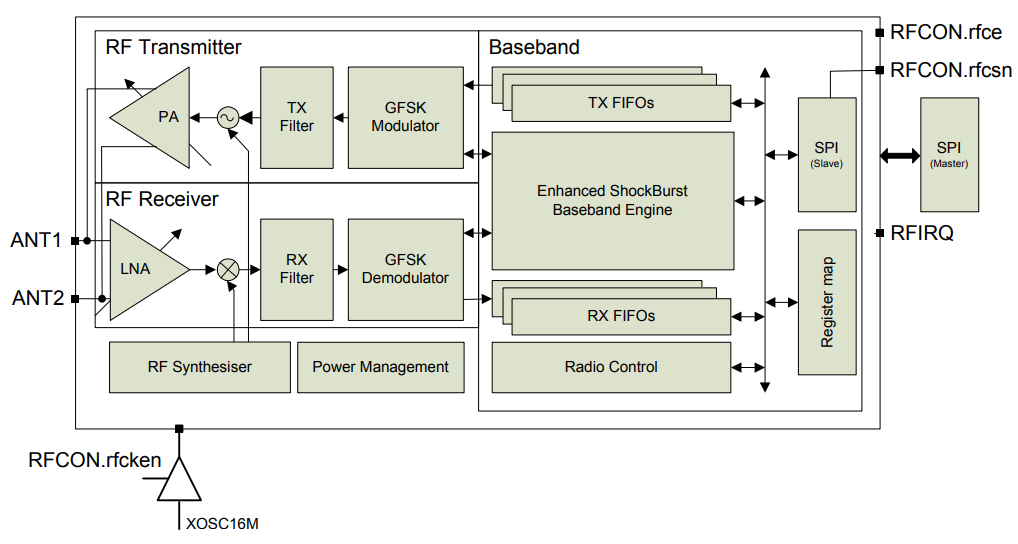
\includegraphics[width=\textwidth]{com_pc2_01.png}
   \caption{Diagrama de Blocos Transceptor RF}
\end{figure}

\subparagraph{Modos de Operação}
O transceptor possui um máquina de estados que controla os diferentes modos de operação. Os modos de operação configuráveis são: (i)Power down, (ii)Standby-I, (iii)Standby-II, (iv)RX e (v)TX. A seguir é mostrado a máquina de estados do transceptor, contido em \citep{bib_com_01_yas}
\begin{figure}[H]
\centering
	\label{com_pc2_02}
	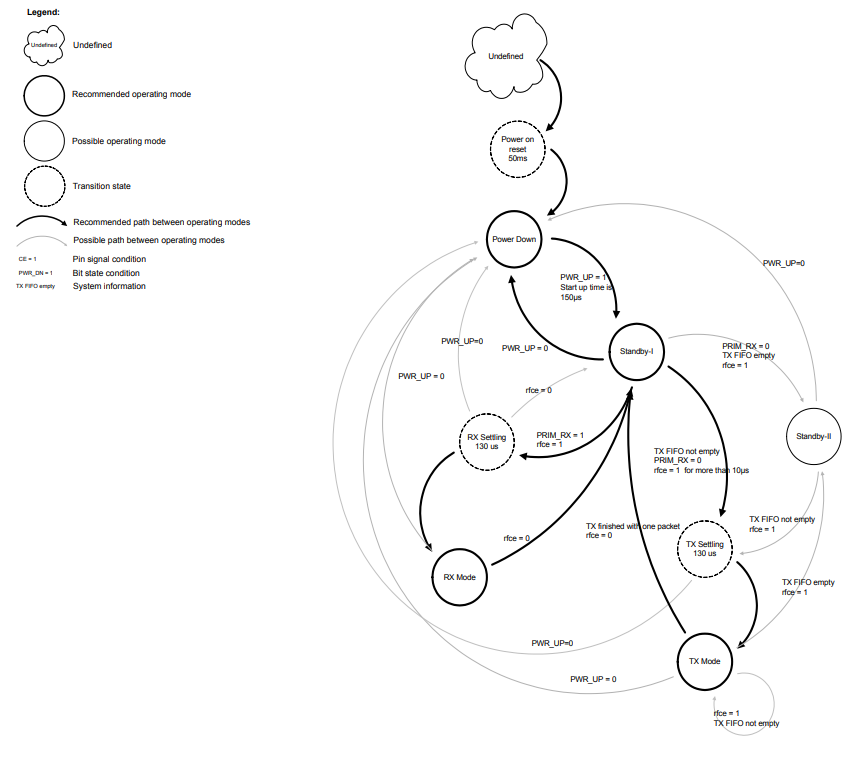
\includegraphics[width=\textwidth]{com_pc2_02.png}
   \caption{Máquina de Estados dos Modos de Operação do Transceptor RF}
\end{figure}

As definições dos modos de operação são:
\begin{itemize}
	\item[Power Down]: O transceptor RF é desabilitado com consumo mínimo de corrente. Todos os valores dos registradores disponíveis pelo SPI são mantidos e o SPI pode ser ativado.
	\item[Standby-I]: Usado para minimizar o consumo médio de corrente e manter tempos curtos de inicialização. O modo ativo ocorre somente se o bit rfce (control enable) estiver ativado, enquanto não estiver, o transceptor de RF retorna ao Standby-I dos modos TX e RX.
	\item[Standby-II]: Nesse modo os buffers de clock extras são ativados e há maior consumo de corrente em comparação com ao (ii). O transceptor de RF entrará no modo de espera II se o bit rfce for mantido alto durante uma uma transmissão com os FIFOs de transmissão (FIFOs TX) vazio. Se um novo pacote é baixado para o FIFO TX, o filtro PLL é iniciado imediatamente e o pacote é transmitido após o atraso normal de estabelecimento do PLL ($\delta t _ {PLL} = 130µs$).
	\item[RX]: Transceptor é ativado como receptor. Nesse modo, o receptor demodula os sinais que chegam no canal, apresentando constantemente os dados demodulados ao mecanismo de protocolo de banda base. Se um pacote válido for encontrado (por um endereço correspondente e um CRC() válido), o payload do pacote será apresentado em um slot livre nos FIFOs de recepção (FIFOs RX). Se os FIFOs RX estiverem cheios, o pacote recebido é descartado.
	O transceptor permanece nesse modo até o microcontrolador configurar os modos (i) ou (ii). Entretanto se o protocolo de enlace (Enhanced ShockBurst^{TM}) estiver habilitado, o transceptor pode assumir outros modos para executar o protocolo.
	\item[TX]: Transceptor é ativado como transmissor e permanece ativo até que não haja mais pacotes a serem transmitidos nos FIFOs TX, se o bit rfce estiver alto, caso contrário o modo TX fica ativo até finalizar a transmissão de um pacote apenas. é importante nunca deixar o transceptor em modo TX por mais de 4ms por vez. Se o protocolo de enlace estiver ativado, o modo TX nunca fica ativo por mais de 4ms.
\end{itemize}

Na tabela \cite{tab_com_pc1_01} é apresentada as configuração dos registradores para cada modo de operação da máquina de estados.
\begin{table}
\begin{tabular}{| c | c | c | c | c |}\hline
Modo & Registrador PWR-UP & Registrador PRIM_RX & rfce & Estado dos FIFOs \\ \hline
RX & 1 & 1 & 1 & - \\ \hline
TX & 1 & 0 & 1 & Esvasia todos os níveis no FIFO TX^a \\ \hline
TX & 1 & 0 & Mínimo de $10\mu s$ de pulso alto & Esvasia apenas um nível no FIFO TX^b \\ \hline
Standby-I & 1 & 0 & 1 & FIFO TX vazio \\ \hline
Standby-II & 1 & - & 0 & Sem pacotes para transmissão a caminho \\ \hline
Power Down & 0 & - & - & - \\ \hline
\end{tabular}
a - Se o bit rfce é mantido alto o FIFO TX é esvaziado e todos os ACK necessarios e possíveis retransmissões são realizados. A transmissão continua enquanto o FIFO TX for recarregado. Se o FIFO de TX estiver vazio quando o bit rfce ainda estiver alto, o transceptor de RF entrará em Standby-II. Neste modo, a transmissão de um pacote é iniciada assim que o rfce é definido alto após o upload de um pacote para o FIFO TX.
b - Este modo de operação realiza um pulso alto no bit rfce por pelo menos 10 $\mu$ s. Permitindo a transmissão de um único pacote. Este é o modo de operação normal, e após a transmissão do pacote, o transceptor de RF entra no Standby-I.
\end{table}

\subparagraph{Frequência do Canal}
A largura de banda ocupada pelo canal depende da taxa de trasmissão usada no transceptor, sendo menor que 1 MHz em 250kbps e 1Mbps e menor que 2 MHz em 2Mbps. O transceptor opera entre 2.4 - 2.525 GHz e a resolução da frequência do canal, programada nas configurações do transceptor, é de 1MHz. Deste modo, para garantir que não haverá overlapping, quando a taxa de transmissão for 2Mbps, o espaçamento no canal deve ser de 2MHz ou mais e, consequentemente, garantindo a mesma condição para as taxas de 250kbps e 1Mbps considerando que a largura de banda de ambas taxas são menores que a resolução de frequência do canal. 

A frequência do canal é inicializada pelo registrador RF_CH de acordo com a fórmula 
$F0= 2400 + RF_CH MHz$
Para comunicação mútua, o receptor e o transmissor devem ter a mesma frequência do canal RF.

\subparagraph{Detector de Potência Recebida (RPD)}
O RPD, localizado no registrador 9 - bit 0, dispara a partir de níveis de potência acima de -64 dBm detectados no canal, caso contrário o RDP = 0.

O RPD pode ser lido a qualquer momento enquanto o transceptor RF estiver em modo RX. Isso oferece um snapshot do nível atual de potência recebida no canal. O RPD é bloqueado sempre que um pacote é recebido ou
quando o microcontrolador define rfce = 0. O status do RPD está correto quando o modo RX está ativado e após um tempo de espera de Tstby2a + Tdelay_AGC = 130us + 40µs. O ganho de RX varia com a temperatura, o que significa que o limiar de RPD também varia temperatura. O threshold de RPD é reduzido em 5dB a T = -40 ° C e aumentado em 5dB a 85 ° C.